\documentclass{article}

\usepackage{graphicx}
\usepackage{tikz}
\usepackage{tikzsymbols}
\usetikzlibrary{calc,patterns,shapes.geometric}
\pagestyle{empty}
\usepackage[margin=0pt]{geometry}
\geometry{papersize={14in,12in}}

\def\centerarc[#1](#2)(#3:#4:#5){\draw[#1] ($(#2)+({#5*cos(#3)},{#5*sin(#3)})$) arc (#3:#4:#5);}

\begin{document}
	\begin{figure}
		\centering
		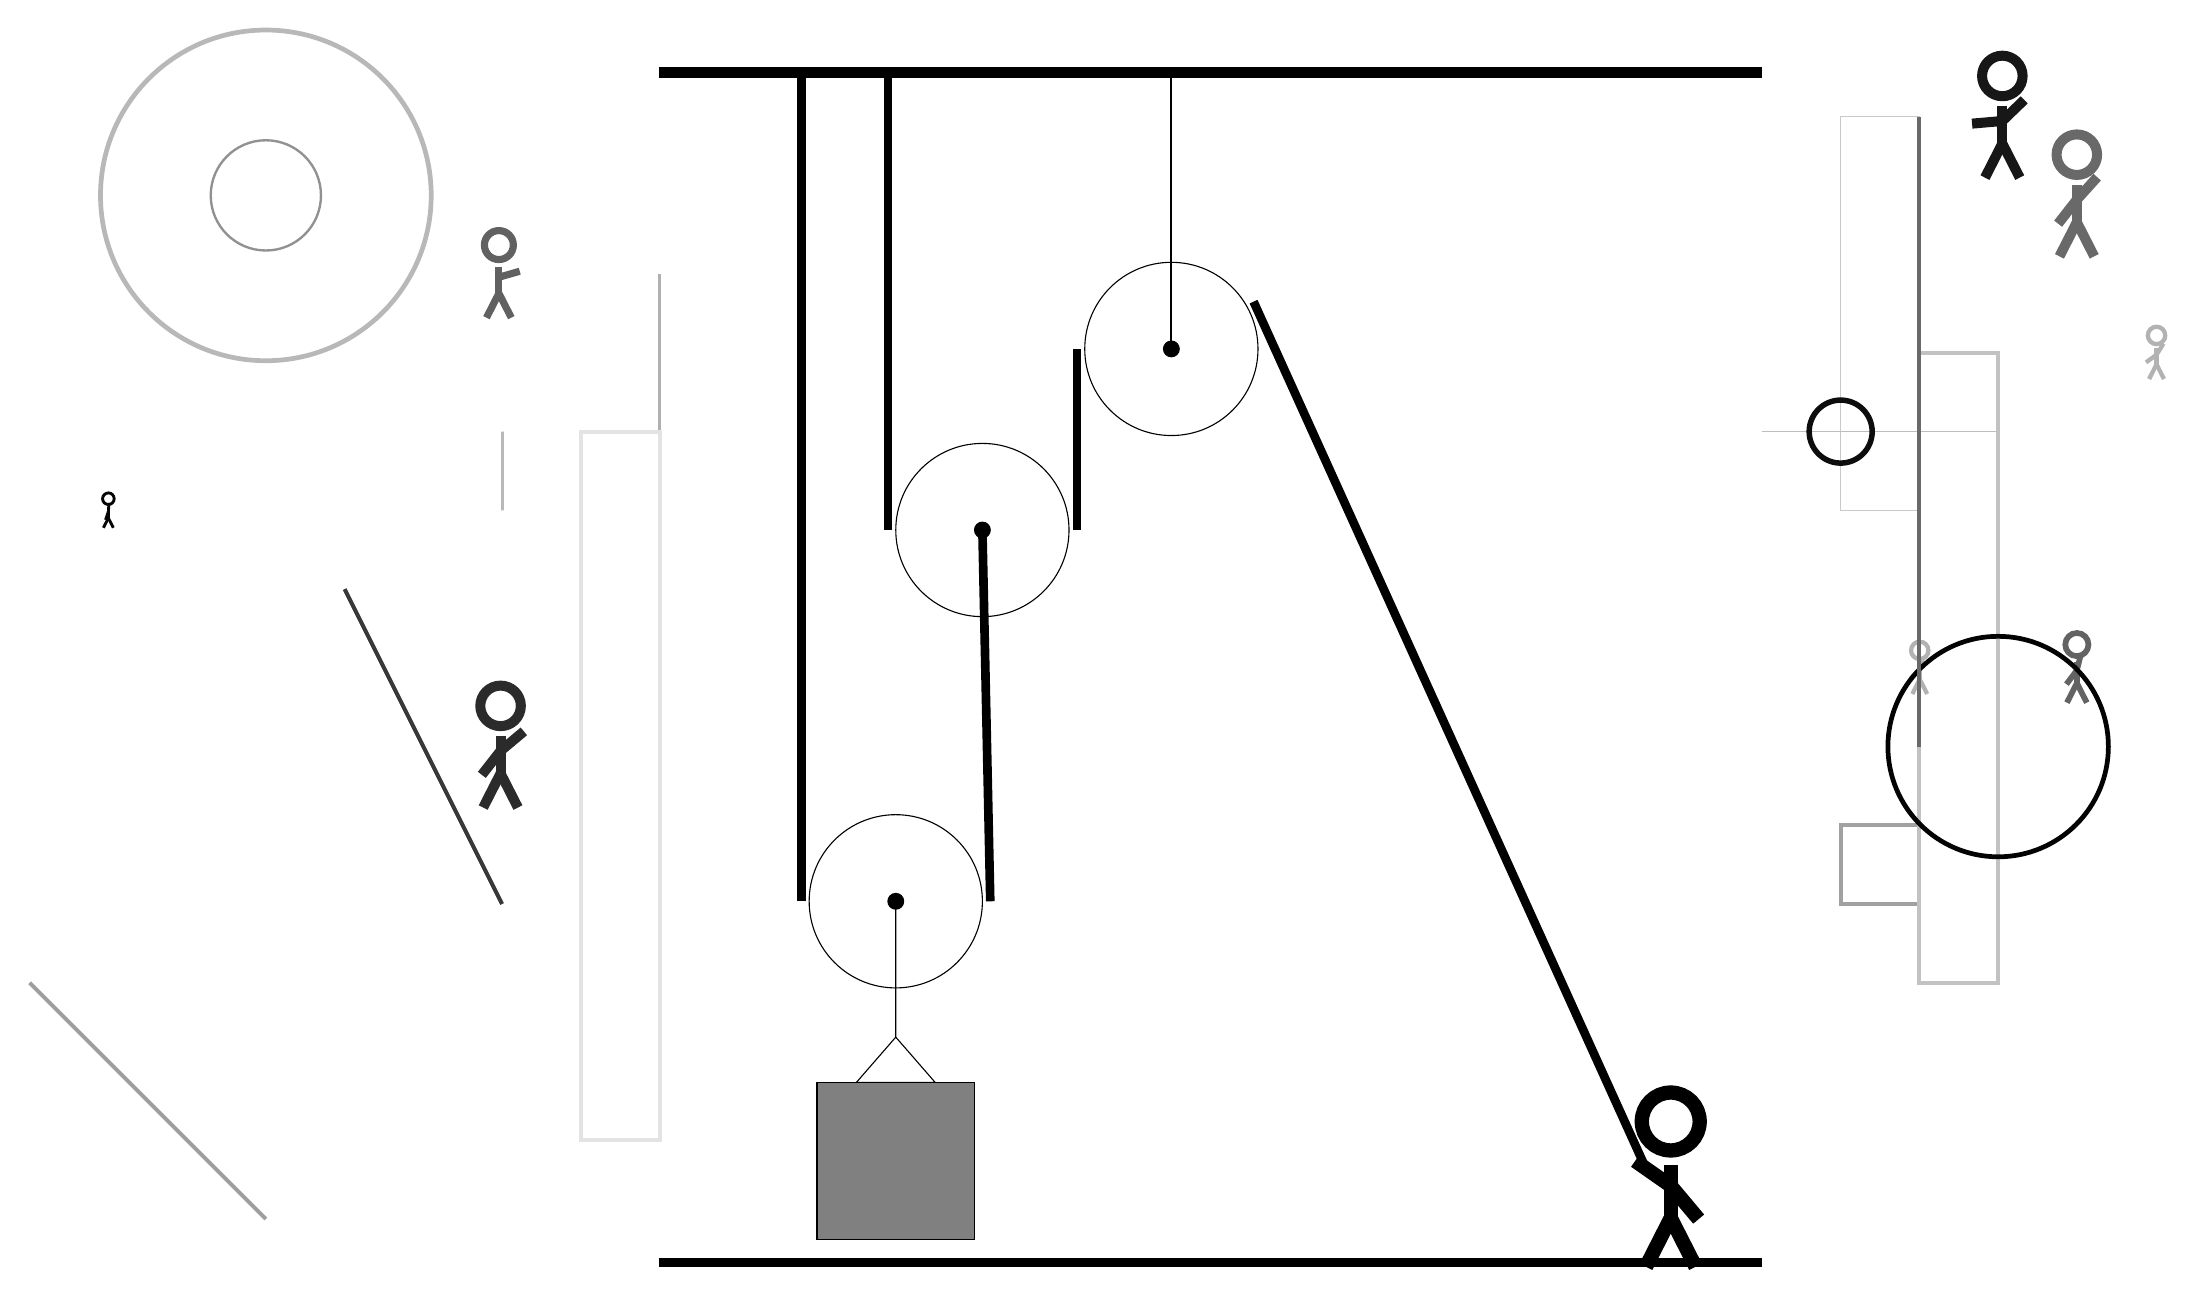
\begin{tikzpicture}
			%%%%% START %%%%%
			
			\draw[fill=black] (-2, 11.5) rectangle (12, 11.625);
			
			\draw (1, 1.035) circle (1.1);
			\draw[fill=black] (1, 1.035) circle (0.1);
			
			\draw (2.1, 5.75) circle (1.1);
			\draw[fill=black] (2.1, 5.75) circle (0.1);
			
			\draw (4.5, 8.05) circle (1.1);
			\draw[fill=black] (4.5, 8.05) circle (0.1);
			\draw[thick] (4.5, 8.05) -- (4.5, 11.5);
			
			\draw[line width=0.2mm, color=black!21] (13, 11) rectangle (14, 6);
			
			\draw[line width=0.5mm, color=black!37] (13, 1) rectangle (14, 2);
			\draw [line width=0.3mm, color=black!43](-7, 10) circle (0.7);
			\node[line width=0.2mm, color=black!30] at (17, 8) {\Strichmaxerl[3][36][58]};
			\node[line width=0.4mm, color=black!30] at (14, 4) {\Strichmaxerl[3][44][76]};
			\draw[line width=0.2mm, color=black!26] (12, 7) rectangle (15, 7);
			
			\node[line width=0.5mm, color=black!83] at (-4, 3) {\Strichmaxerl[7][52][40]};
			\node[line width=0.7mm, color=black!91] at (15, 11) {\Strichmaxerl[7][5][44]};
			\node[line width=0.4mm, color=black!98] at (-9, 6) {\Strichmaxerl[2][71][86]};
			
			\draw [line width=0.6mm, color=black!28](-7, 10) circle (2.1);
			\node[line width=0.3mm, color=black!59] at (16, 10) {\Strichmaxerl[7][52][48]};
			\draw[line width=0.5mm, color=black!24] (14, 8) rectangle (15, 0);
			\draw[line width=0.5mm, color=black!38](-7, -3) -- (-10, 0);
			
			\draw[line width=0.7mm, color=black!27] (-4, -1) rectangle (-4, -1);
			\draw[line width=0.4mm, color=black!28] (-4, 6) rectangle (-4, 7);
			\draw [line width=0.7mm, color=black!95](13, 7) circle (0.4);
			\draw[line width=0.3mm, color=black!31] (-2, 9) rectangle (-2, 7);
			\node[line width=0.2mm, color=black!61] at (16, 4) {\Strichmaxerl[4][53][76]};
			\node[line width=0.2mm, color=black!62] at (-4, 9) {\Strichmaxerl[5][90][16]};
			\draw[line width=0.5mm, color=black!11] (-3, -2) rectangle (-2, 7);
			\draw [line width=0.6mm, color=black!99](15, 3) circle (1.4);
			
			\draw [line width=0.6mm, color=black!46](-6, 10) circle (0.0);
			\draw[line width=0.5mm, color=black!78](-6, 5) -- (-4, 1);
			\draw[line width=0.5mm, color=black!59](14, 3) -- (14, 11);
			
			\draw (1, 1.035) -- (1, -0.69) -- (0.5, -1.265) -- (1.5, -1.265) -- (1, -0.69);
			\draw[fill=black!50] (0, -1.265) rectangle (2, -3.265);
			
			\draw[line width=1.1mm] (-0.2, 11.5) -- (-0.2, 1.035);
			\centerarc[line width=1.1mm](1, 1.035)(180:360:1.2000000000000002);
			\draw[line width=1.1mm](2.2, 1.035) -- (2.1, 5.75);
			\draw[line width=1.1mm] (0.9, 11.5) -- (0.9, 5.75);
			\centerarc[line width=1.1mm](2.1, 5.75)(180:360:1.2000000000000002);
			\draw[line width=1.1mm](3.3, 5.75) -- (3.3, 8.05);
			\centerarc[line width=1.1mm](4.5, 8.05)(30:180:1.2000000000000002);
			\draw[line width=1.1mm] (5.544, 8.65) -- (10.5, -2.3);
			
			\node at (10.8, -2.5) {\Strichmaxerl[10][-35][-50]};
			
			\draw[fill=black] (-2, -3.5) rectangle (12, -3.6);
			
			%%%%% END %%%%%
		\end{tikzpicture}
	\end{figure}	
\end{document}